\section{Count-Min Sketching Using Hashing}

\paragraph{The main idea of Count-Min Sketching is to use multiple hash functions to count the frequency of keys.\\
We have a large stream of keys and we will keep a counter in order to record the apprearance of each key.\\
There are two counts involved in this concept: the real count and the appoximate count.\\
Let's take a look at a simple example.\\
We would like to keep count of how ofter each URL in a given web server is requested.\\}

\begin{figure}[H]
    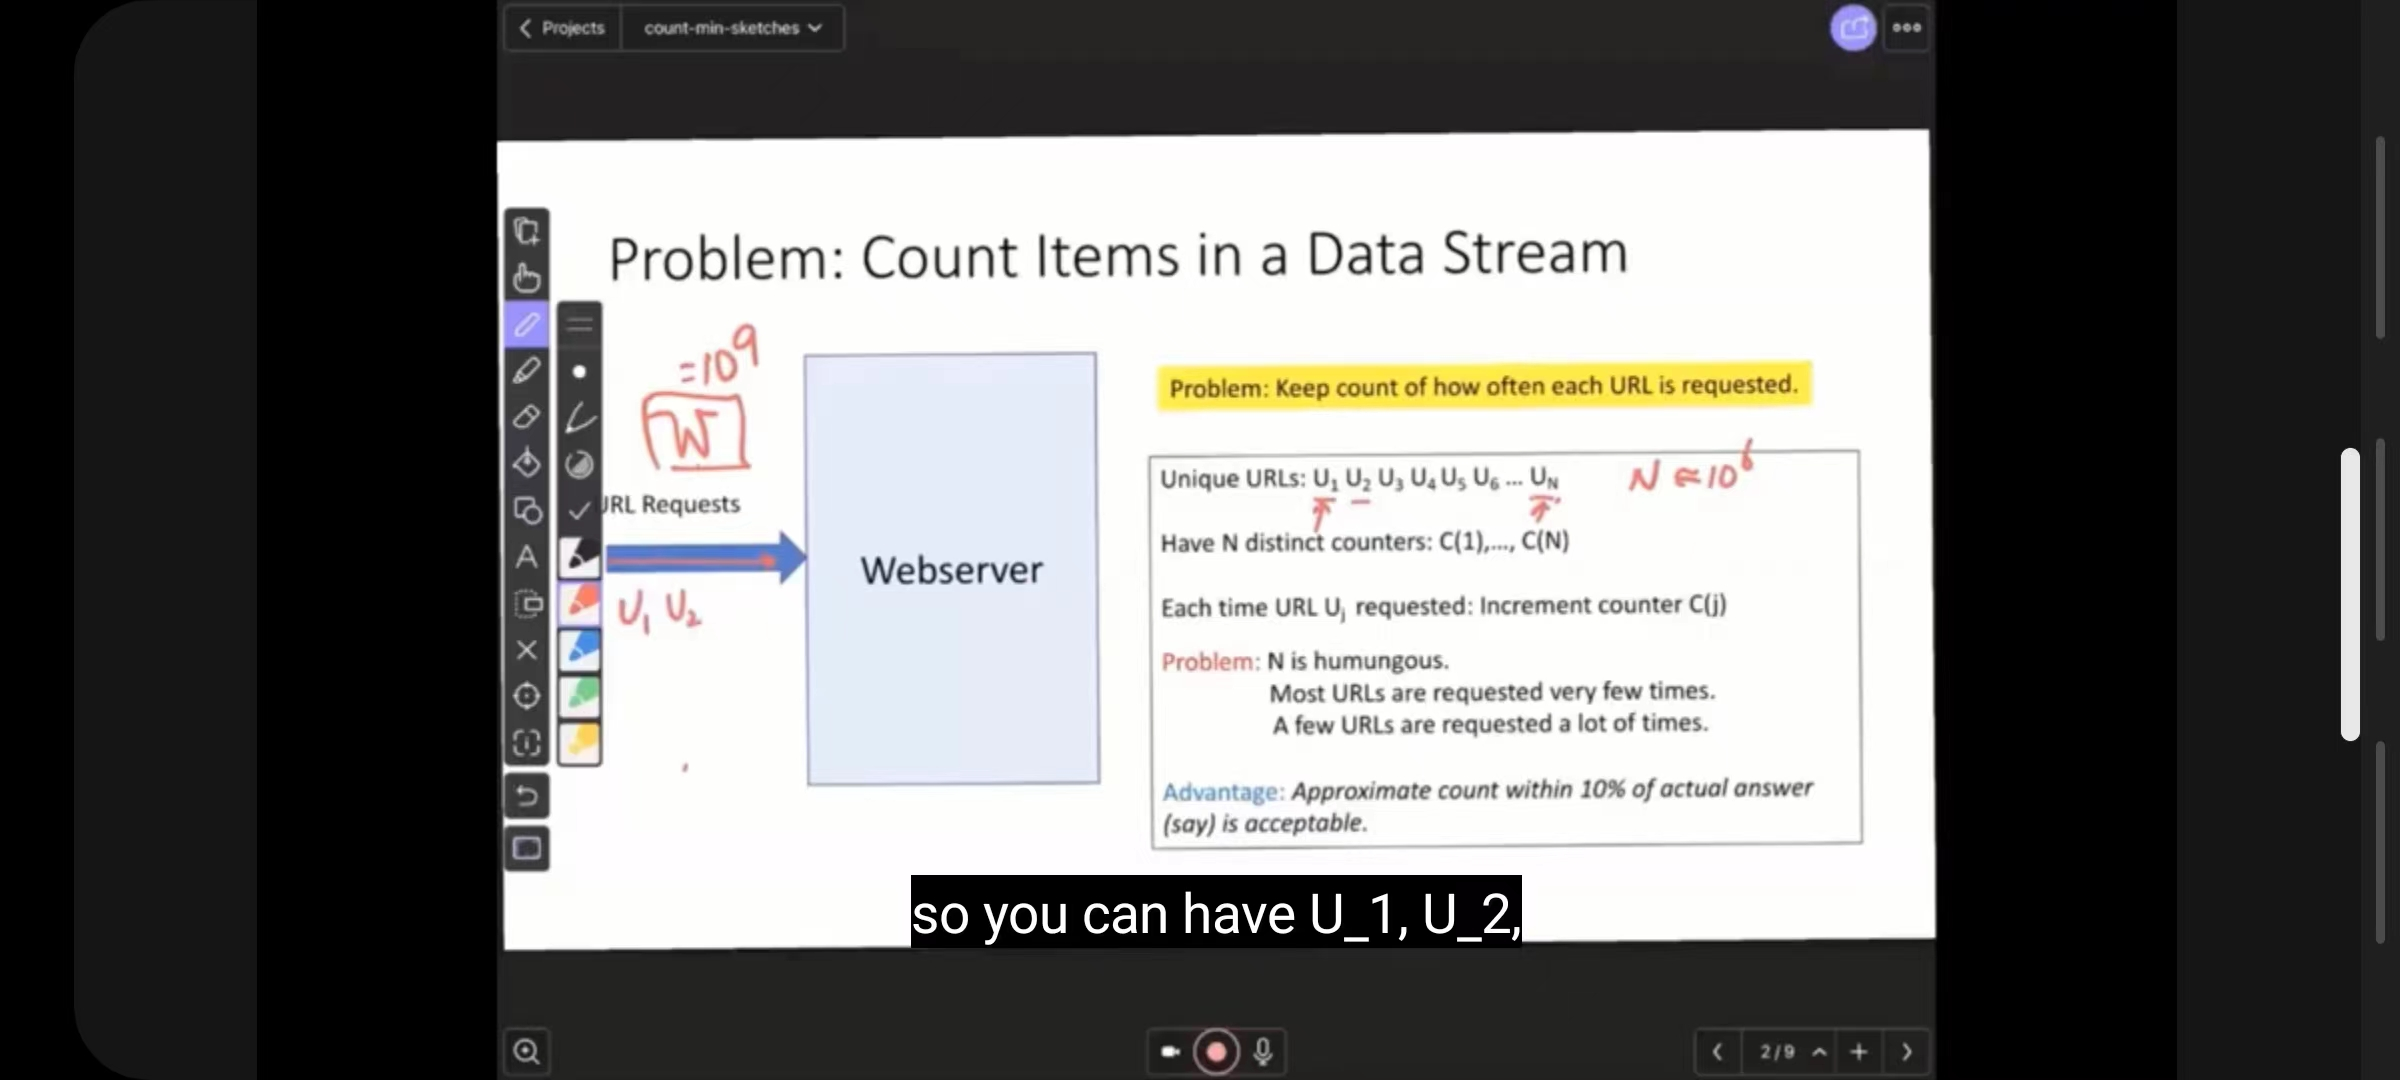
\includegraphics[width=\textwidth]{webserver.jpg}
\end{figure}

\paragraph{
    For each time we get a request, we will hash the URL and increase the counter by 1.\\
    Let's say URL $U_j$ is hashed into slot $h_i(U_j)$, and we will increase the counter $C(j)$ by 1.\\
}

\subsection{Approximate Counting Data Structure}

\begin{figure}[H]
    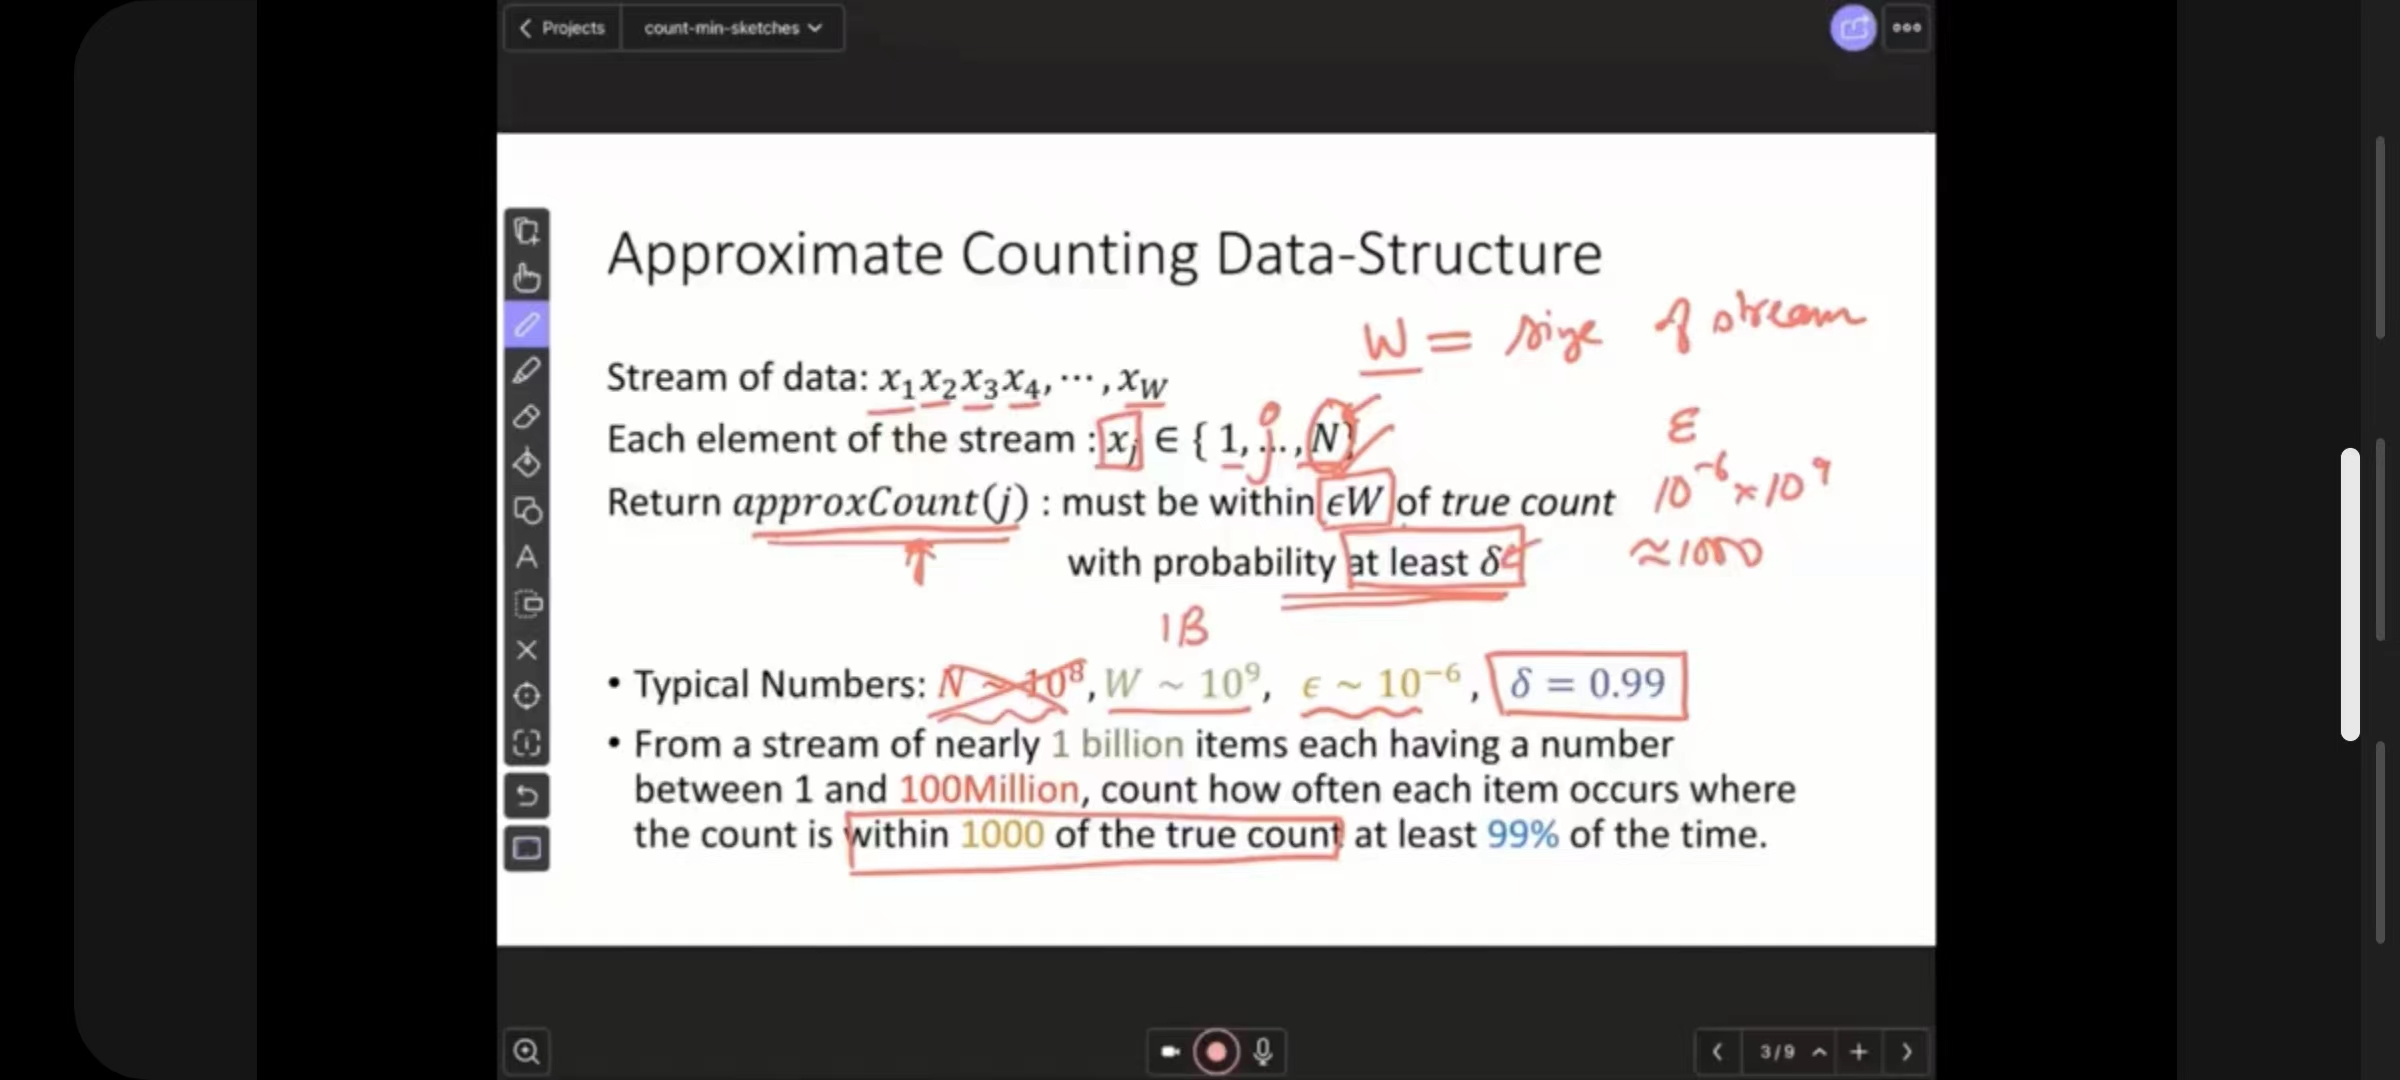
\includegraphics[width=\textwidth]{appoximatecountingdatastructure.jpg}
\end{figure}

\paragraph{
    Let's take a look at a stream of elements ${x_1, x_2, \ldots ,x_w}$ in which $w$ is the size of the stream.\\
    Each element $x_j \in {1,2,\ldots,n}$ (The number type is just an example, it can be any type), 
    therefore there'll be $n$ possibilities of $x_j$.\\
    In order to get an appoximate count, the returned value must be within the range of $\epsilon*w$, where $\epsilon$
    is a relatively small number.\\
    And the probability of approximate count must larger than $\delta$.\\
    Here are the typical number choice for above variables:\\
    $w \approx 10^9,n \approx 10^8, \epsilon \approx 10^{-6}, \delta \approx 0.99$.\\
}

\paragraph{
    Let's dive into the basic idea of Count-Min Sketching.\\
    We will use $m$ counters: $C(1), \ldots, C(m)$.\\
    Once we encounter an element $X(j)$, we will hash it into $m$ slots, a.k.a. $h_1(X(j)), \ldots, h_m(X(j))$.\\
    Then we will increase the counters in the corresponding slots, such as $C(j)$, by 1.\\
    As this mechanism goes on, we will have multiple hashes that are the same, and the counter will be increased by 1 multiple times
    (that is to say, multiple hashes may point to the same $C(j)$);\\
}

\begin{figure}[H]
    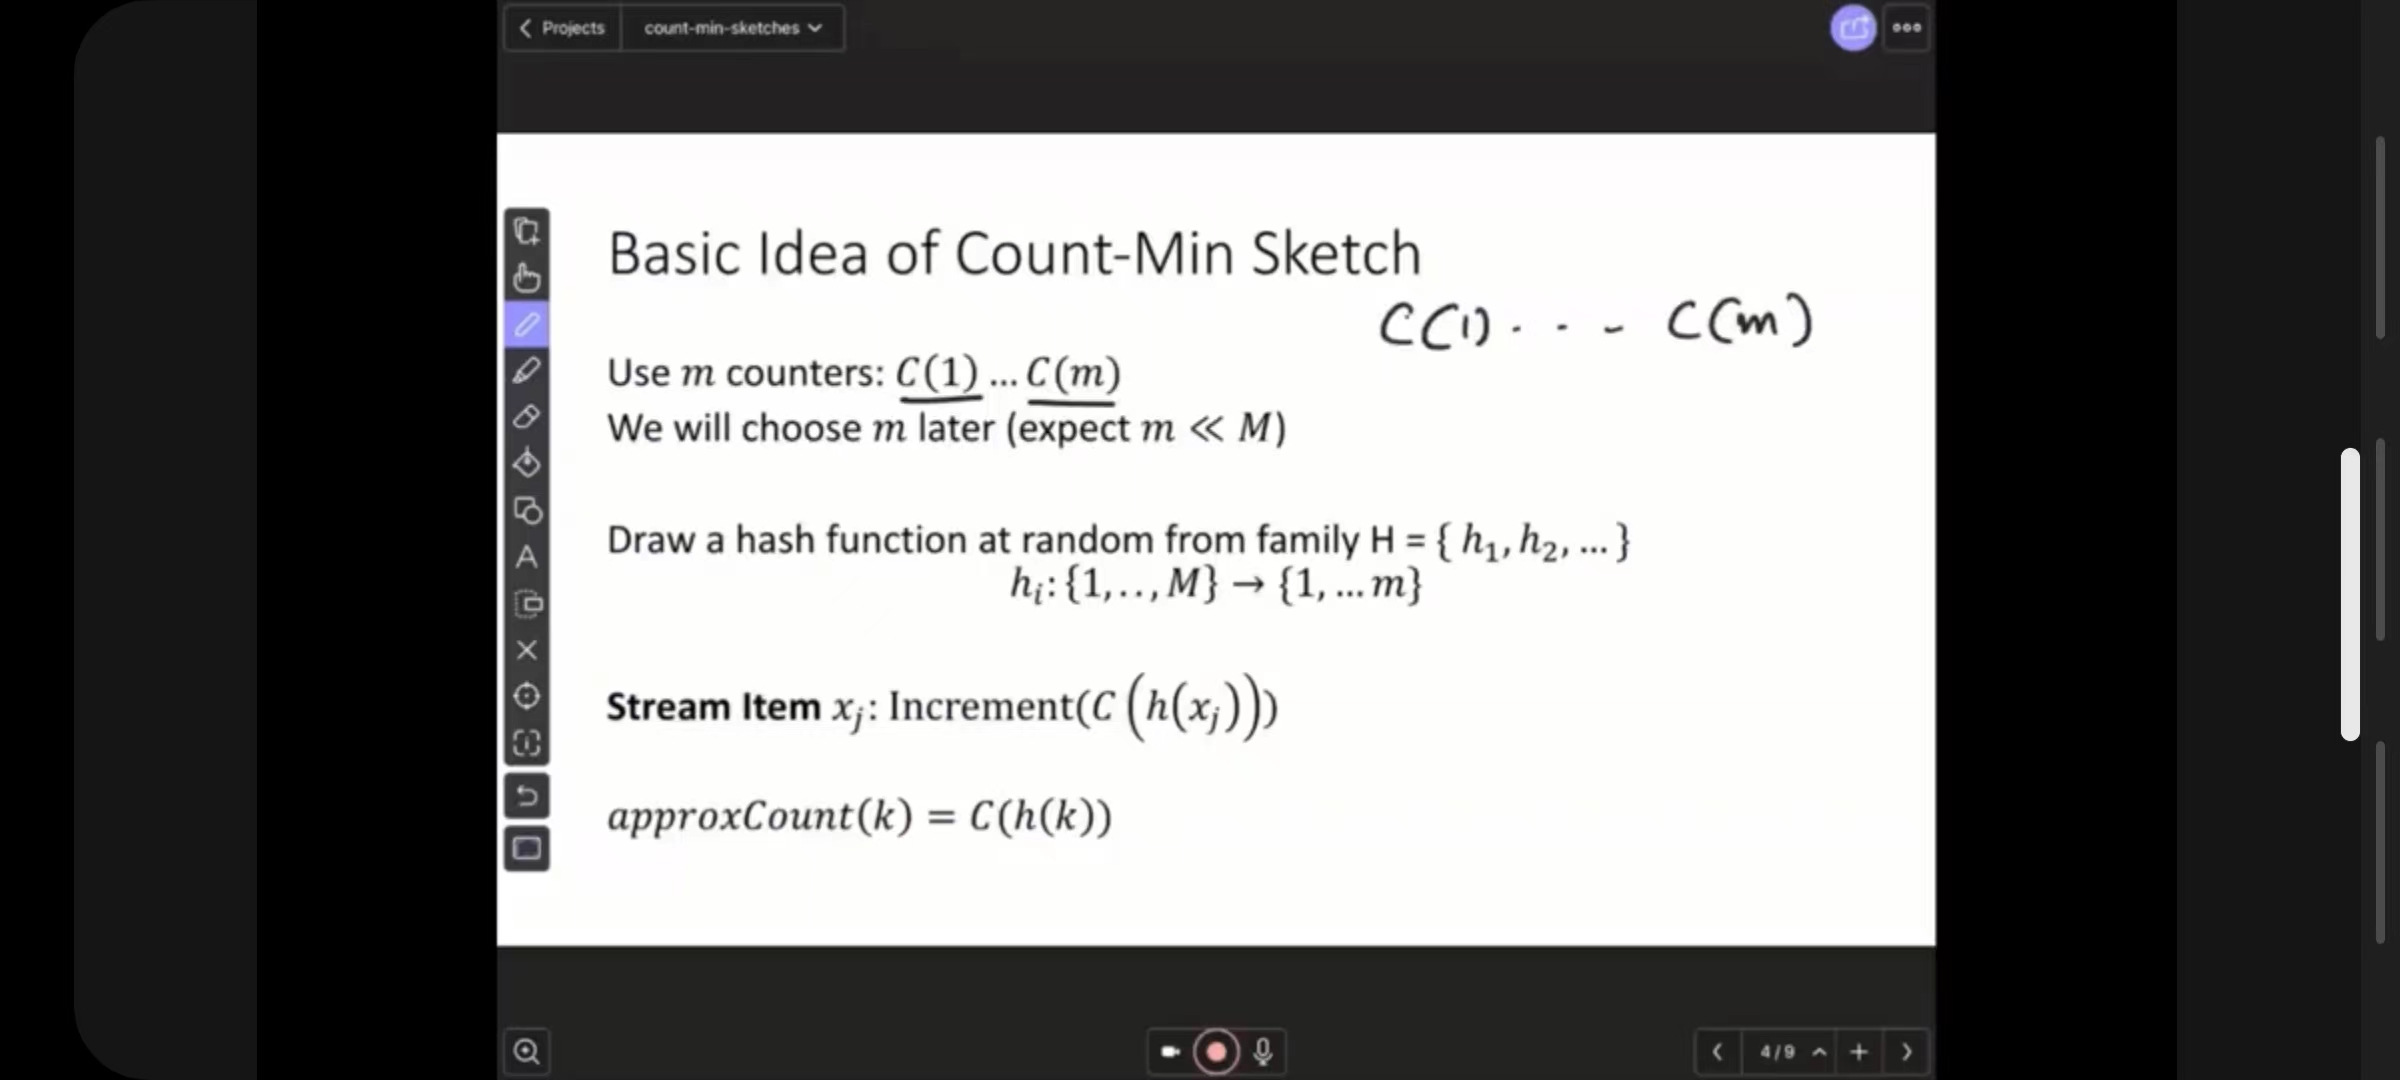
\includegraphics[width=\textwidth]{countminsketchbasicidea.jpg}
\end{figure}

\begin{verbatim}
    Xj -> Cj
    Xm -> Cj
    Xn -> Cj
\end{verbatim}

\subsection{Count-Min Sketch Error Analysis}

\paragraph{
    We know that the approximate count generally is larger than the real count. But how do they relate to each other?\\
    The probability that $h(j) = h(i)$ under certain hash function is as following;\\
    $Pr(h(i)=h(j)) = c/m, h \in H, i \neq j$\\
    Typically, $c=1$.\\
    Then the expected value of appoximatecount(j) is as following;\\
    $E[appoximatecount(j)] = \sum_{i=1}^n Pr(h(i)=h(j)) * realcount(i) = \sum_{i=1}^n c/m * realcount(i)$;\\
    And it's $\leq realcount(j) + c*w/m$.\\
    Therefore, the `error` in the analysis is denoted as;\\
    $error = appoximatecount(j) - realcount(j) \leq c*w/m$.\\
}